\documentclass[11pt,a4paper]{article}

% ── Packages ──
\usepackage[utf8]{inputenc}
\usepackage[T1]{fontenc}
\usepackage[margin=1in]{geometry}
\usepackage{amsmath,amssymb,amsfonts}
\usepackage{booktabs}
\usepackage{longtable}
\usepackage{enumitem}
\usepackage{graphicx}
\usepackage{xcolor}
\usepackage{hyperref}
\usepackage{tikz}
\usetikzlibrary{shapes.geometric, arrows.meta, positioning, fit, calc}
\usepackage{algorithm}
\usepackage{algpseudocode}
\usepackage{multicol}
\usepackage{caption}
\usepackage{subcaption}
\usepackage{fancyhdr}
\usepackage{titlesec}
\usepackage{tcolorbox}
\usepackage{float}
\usepackage{tabularx}
\usepackage{array}

% ── Colors ──
\definecolor{metu}{RGB}{120,0,0}
\definecolor{accentblue}{RGB}{0,80,158}
\definecolor{boxgray}{RGB}{245,245,248}
\definecolor{darkgreen}{RGB}{0,120,60}

% ── Hyperref config ──
\hypersetup{
    colorlinks=true,
    linkcolor=metu,
    citecolor=accentblue,
    urlcolor=accentblue
}

% ── Header/Footer ──
\pagestyle{fancy}
\fancyhf{}
\fancyhead[L]{\small\textcolor{metu}{CENG 488 --- Guided Research}}
\fancyhead[R]{\small\textcolor{metu}{METU --- Spring 2026}}
\fancyfoot[C]{\thepage}
\renewcommand{\headrulewidth}{0.4pt}

% ── Section formatting ──
\titleformat{\section}{\Large\bfseries\color{metu}}{\thesection}{1em}{}
\titleformat{\subsection}{\large\bfseries\color{metu!80!black}}{\thesubsection}{1em}{}
\titleformat{\subsubsection}{\normalsize\bfseries\color{metu!60!black}}{\thesubsubsection}{1em}{}

% ── Custom boxes ──
\newtcolorbox{keyinsight}{
    colback=accentblue!5,
    colframe=accentblue!60,
    fonttitle=\bfseries,
    title=Key Insight,
    sharp corners,
    boxrule=0.5pt
}

\newtcolorbox{designchoice}{
    colback=darkgreen!5,
    colframe=darkgreen!60,
    fonttitle=\bfseries,
    title=Design Choice,
    sharp corners,
    boxrule=0.5pt
}

\newtcolorbox{warningbox}{
    colback=red!5,
    colframe=red!60,
    fonttitle=\bfseries,
    title=Critical Consideration,
    sharp corners,
    boxrule=0.5pt
}

% ── Document ──
\begin{document}

% ════════════════════════════════════════
% TITLE PAGE
% ════════════════════════════════════════
\begin{titlepage}
\centering
\vspace*{1cm}

{\Huge\bfseries\textcolor{metu}{What Do Options Markets Know?}\par}
\vspace{0.6cm}
{\LARGE\textcolor{metu!80!black}{Explainable Deep Learning for}\par}
{\LARGE\textcolor{metu!80!black}{Options-Based Equity Return Prediction}\par}

\vspace{1.5cm}

{\Large CENG 488 --- Guided Research\par}
{\Large Comprehensive Project Document\par}

\vspace{1cm}

{\large Department of Computer Engineering\par}
{\large Middle East Technical University\par}

\vspace{1cm}
{\large February 2026\par}

\vspace{2cm}


\begin{tikzpicture}
\draw[metu, ultra thick] (0,0) -- (12,0);
\end{tikzpicture}

\vspace{1cm}

\begin{abstract}
\noindent This document provides a comprehensive, self-contained specification of a guided research project that investigates whether options market data contains predictive information about future equity returns. We use a suite of machine learning models---feedforward neural networks, gradient-boosted trees (XGBoost), Temporal Fusion Transformers (TFT), and TabNet---trained on a rich set of options-derived features to forecast next-day stock returns for major US equities. The core contribution is an explainability analysis using SHAP, TFT variable selection gates, and TabNet attention masks to identify \emph{which} options signals predict stock movement, \emph{when} they are most informative (across market regimes, earnings cycles, and liquidity conditions), and \emph{how} they interact. The project also incorporates recent developments in quantitative finance, including dealer gamma exposure, options-implied higher moments, zero-days-to-expiration (0DTE) activity metrics, and LLM-derived news sentiment. This document covers every aspect of the project: motivation, theoretical background, problem formulation, complete feature engineering, model architectures, training procedures, explainability methods, evaluation framework, data pipeline, timeline, and potential extensions.
\end{abstract}

\end{titlepage}

\tableofcontents
\newpage

% ════════════════════════════════════════
% 1. INTRODUCTION
% ════════════════════════════════════════
\section{Introduction and Motivation}

\subsection{The Central Question}

Options markets are where informed traders go. An investor with private information that a stock will decline has strong incentives to buy put options rather than short the stock: options provide leverage (a small premium controls a large notional position), limited downside (the maximum loss is the premium paid), and relative anonymity in a fragmented market. This asymmetry implies that \textbf{options market activity should contain forward-looking information about underlying equity prices that is not yet fully reflected in the stock price itself}.

This hypothesis---that options markets lead stock markets in price discovery---is well-established in academic finance. Easley, O'Hara, and Srinivas (1998) showed that options volume predicts stock returns. Pan and Poteshman (2006) demonstrated that the put-call ratio constructed from signed options volume (distinguishing buyer-initiated from seller-initiated trades) predicts equity returns. Cremers and Weinbaum (2010) found that deviations from put-call parity predict cross-sectional stock returns. An and Ang (2012) showed that changes in implied volatility predict returns.

However, each of these studies examines one or two options-derived signals in isolation. No comprehensive study has taken a rich, multi-dimensional set of options features and used modern explainable machine learning to systematically identify: (1) which options signals carry the most predictive information, (2) when and under what conditions this information is strongest, and (3) how these signals interact with each other and with broader market conditions.

This gap is what our project fills.

\subsection{Why This Matters}

\begin{keyinsight}
If options market data predicts stock returns, this has implications far beyond options trading. Every equity investor, portfolio manager, risk manager, and algorithmic trader can benefit from understanding what the options market ``knows'' about future stock movements. The audience for these findings is the entire financial ecosystem.
\end{keyinsight}

The question matters for three reasons:

\textbf{Market efficiency.} If options signals predict stock returns even after controlling for standard risk factors and stock-level information, this challenges the semi-strong form of the Efficient Market Hypothesis, which holds that all publicly available information is already reflected in stock prices.

\textbf{Price discovery.} Understanding where and when information enters the market is a foundational question in market microstructure. Our analysis can reveal whether information flows from options to stocks (options lead), from stocks to options (stocks lead), or bidirectionally, and how this depends on market conditions.

\textbf{Practical value.} Even modest predictability---an $R^2$ of 0.01--0.05 at the daily horizon---can be economically significant when translated into a systematic trading strategy. Our explainability analysis can guide practitioners on \emph{when} to trust options-derived signals and when to ignore them.

\subsection{Why Explainability Is Essential}

A model that predicts stock returns 2\% more accurately than a baseline is of limited value if no one understands what it has learned. In finance, black-box predictions face three specific challenges:

\textbf{Regulatory and institutional trust.} Asset managers must justify their investment decisions to clients and regulators. ``The neural network told us to buy'' is not an acceptable explanation.

\textbf{Regime robustness.} A model trained on calm-market data may fail catastrophically in a crisis if its learned relationships are regime-specific. Explainability reveals whether the model relies on features that are stable vs.\ features that are regime-dependent, enabling risk management.

\textbf{Scientific contribution.} The goal of this research is not merely to build a better prediction machine, but to advance our understanding of how information flows through financial markets. Explainability transforms a prediction model into a tool for scientific discovery.


% ════════════════════════════════════════
% 2. THEORETICAL BACKGROUND
% ════════════════════════════════════════
\section{Theoretical Background}

\subsection{Option Pricing and the Black--Scholes Framework}

The Black--Scholes model (Black \& Scholes, 1973) prices a European call option as:
\begin{equation}
C = S \cdot N(d_1) - K \cdot e^{-rT} \cdot N(d_2)
\end{equation}
where
\begin{equation}
d_1 = \frac{\ln(S/K) + (r + \sigma^2/2)T}{\sigma\sqrt{T}}, \quad d_2 = d_1 - \sigma\sqrt{T}
\end{equation}
and $N(\cdot)$ is the cumulative standard normal distribution. The five inputs are the stock price $S$, strike price $K$, time to expiration $T$, risk-free rate $r$, and volatility $\sigma$.

The model assumes: constant volatility, log-normal returns, continuous trading, no transaction costs, and no dividends (in the basic form). Every one of these assumptions is violated in practice, producing systematic mispricings visible as the volatility smile and skew.

\subsection{Implied Volatility and Information Content}

Implied volatility (IV) is obtained by inverting the Black--Scholes formula: given an observed market price, what value of $\sigma$ makes the model output match the market price? IV is the market's consensus expectation of future realized volatility, embedded in option prices.

Crucially, IV is \emph{forward-looking}. It aggregates the collective expectations of all market participants---including those with private information. This is why IV changes can predict future stock movements: a sudden spike in IV may reflect informed traders positioning for an anticipated event.

\subsection{The Greeks as Sensitivity Measures}

The Greeks describe how option prices respond to changes in the underlying parameters:

\begin{table}[H]
\centering
\begin{tabular}{@{}lll@{}}
\toprule
\textbf{Greek} & \textbf{Definition} & \textbf{Interpretation} \\
\midrule
Delta ($\Delta$) & $\partial C / \partial S$ & Price sensitivity to stock movement \\
Gamma ($\Gamma$) & $\partial^2 C / \partial S^2$ & Convexity / acceleration of delta \\
Theta ($\Theta$) & $\partial C / \partial T$ & Time decay per day \\
Vega ($\nu$) & $\partial C / \partial \sigma$ & Sensitivity to volatility changes \\
Rho ($\rho$) & $\partial C / \partial r$ & Sensitivity to interest rate changes \\
\bottomrule
\end{tabular}
\caption{The option Greeks and their interpretations.}
\end{table}

For our project, the Greeks are relevant not as features of individual contracts (since we aggregate across the options chain), but as tools for computing aggregate measures like net delta exposure and total gamma exposure.

\subsection{Informed Trading in Options Markets}

The theoretical basis for why options data should predict stock returns rests on several pillars:

\textbf{Leverage.} Options provide leveraged exposure: a 1\% move in the stock might produce a 10--50\% move in the option, depending on delta. Informed traders with capital constraints prefer options.

\textbf{Limited downside.} A long option position can lose at most the premium paid. Short-selling stock has theoretically unlimited loss potential.

\textbf{Anonymity and fragmentation.} Options markets are fragmented across multiple exchanges, making it harder to detect large informed orders compared to the consolidated equity market.

\textbf{Directional and volatility bets.} Options allow traders to express views not just on direction (up/down) but on volatility (big move vs.\ small move) and timing (before/after an event). This richer information set is embedded in options prices.

\subsection{Dealer Gamma Exposure and Mechanical Price Impact}

Market makers (dealers) who sell options to end-users must delta-hedge their exposure by trading the underlying stock. The direction and intensity of this hedging depends on the dealers' aggregate gamma exposure (GEX):

\textbf{When dealers are long gamma} (net positive gamma), they hedge by \emph{selling into rallies and buying into dips}, dampening stock price movements. This creates a mean-reverting force.

\textbf{When dealers are short gamma} (net negative gamma), they hedge by \emph{buying into rallies and selling into dips}, amplifying stock price movements. This creates a momentum/trend-following force.

\begin{keyinsight}
Dealer gamma exposure creates a \emph{mechanical} link between the options market and stock prices that is distinct from the \emph{informational} channel. Our model can potentially disentangle these two channels through SHAP interaction analysis.
\end{keyinsight}

\subsection{The Rise of 0DTE Options}

Zero-days-to-expiration (0DTE) options---contracts that expire on the same day they are traded---now account for approximately 40--50\% of S\&P 500 options volume. This structural shift, which accelerated in 2022--2023, has several implications:

\begin{itemize}[nosep]
    \item Massive intraday gamma exposure for market makers, creating amplified hedging flows
    \item New source of information: 0DTE volume reflects very short-term directional views
    \item Increased ``pinning'' behavior around round strike prices near the close
    \item Potential for gamma-driven feedback loops that amplify intraday stock volatility
\end{itemize}

Including 0DTE-related features (aggregate near-expiry volume, 0DTE-specific IV levels) captures a signal that barely existed before 2022 and is still underexplored in the literature.


% ════════════════════════════════════════
% 3. PROBLEM FORMULATION
% ════════════════════════════════════════
\section{Problem Formulation}

\subsection{Primary Target: Next-Day Stock Return}

For each stock $i$ on trading day $t$, we construct a feature vector $\mathbf{x}_{i,t} \in \mathbb{R}^{d}$ from all observable options and stock market information on day $t$. The primary target variable is the next-day stock return:
\begin{equation}
r_{i,t+1} = \frac{S_{i,t+1} - S_{i,t}}{S_{i,t}}
\end{equation}
where $S_{i,t}$ is the closing price of stock $i$ on day $t$.

\begin{designchoice}
We predict \emph{returns} rather than \emph{prices} for three reasons: (1) returns strip out the level effect---a \$200 stock and a \$20 stock become comparable; (2) returns are approximately stationary, which is a requirement for most ML models; (3) a model that predicts returns must learn actual \emph{dynamics}, not merely memorize that tomorrow's price is close to today's price.
\end{designchoice}

\subsection{Secondary Target: Black--Scholes Residual}

As a secondary analysis, we predict the deviation of the actual stock return from what the options market's implied distribution would suggest:
\begin{equation}
\epsilon_{i,t+1} = r_{i,t+1} - \mathbb{E}_{\text{implied}}[r_{i,t+1}]
\end{equation}
where the implied expected return can be approximated from the options-implied risk-neutral density. In practice, we approximate this by predicting the residual of the stock return after removing the component explained by a simple model using only Black--Scholes inputs. This formulation isolates the information in options data that goes \emph{beyond} what standard option-pricing theory captures.

\subsection{Classification Variant: Return Direction}

As a complementary analysis, we also predict the \emph{direction} of next-day returns:
\begin{equation}
y_{i,t+1} = 
\begin{cases}
1 & \text{if } r_{i,t+1} > 0 \\
0 & \text{if } r_{i,t+1} \leq 0
\end{cases}
\end{equation}

This binary classification task allows us to report accuracy, precision, recall, F1, and AUC-ROC, which are more intuitive metrics for assessing directional predictability.

\subsection{Forecasting Horizons}

The primary horizon is one trading day (close-to-close). We additionally explore:
\begin{itemize}[nosep]
    \item \textbf{Overnight return} (close-to-open): Tests whether options signals predict the overnight gap, where institutional information is often revealed.
    \item \textbf{Intraday return} (open-to-close): Tests whether options signals predict same-day trading dynamics.
    \item \textbf{3-day and 5-day returns}: Measures how prediction quality degrades with horizon.
\end{itemize}


% ════════════════════════════════════════
% 4. COMPLETE FEATURE ENGINEERING
% ════════════════════════════════════════
\section{Complete Feature Engineering}

Our feature set is organized into seven categories. Because we are predicting \emph{stock} returns (not individual option prices), all options-derived features must be \emph{aggregated} across the entire options chain for each stock on each day. This aggregation step is a critical design choice documented in Section~\ref{sec:aggregation}.

\subsection{Category 1: Aggregate Options Sentiment Indicators}

These features summarize the directional positioning of all options market participants.

\begin{longtable}{@{}cp{3cm}p{8cm}@{}}
\toprule
\textbf{\#} & \textbf{Feature} & \textbf{Rationale} \\
\midrule
\endfirsthead
\toprule
\textbf{\#} & \textbf{Feature} & \textbf{Rationale} \\
\midrule
\endhead
1 & Put-call volume ratio & Ratio of total put volume to total call volume for the stock on day $t$. A high ratio signals aggregate bearish sentiment. This is one of the most studied single-signal options predictors (Pan \& Poteshman, 2006). \\
\addlinespace
2 & Put-call open interest ratio & Ratio of total put open interest to call open interest. Unlike volume (which measures flow), OI measures \emph{stock} of outstanding positions. A rising put-call OI ratio indicates accumulating bearish positioning. \\
\addlinespace
3 & Options-to-stock volume ratio & Total options volume (in share-equivalent terms, i.e., contracts $\times$ 100) divided by stock trading volume. High values indicate elevated options activity relative to the underlying, which may signal informed trading. \\
\addlinespace
4 & Net delta exposure & $\sum_{j \in \text{calls}} \Delta_j \cdot OI_j - \sum_{j \in \text{puts}} |\Delta_j| \cdot OI_j$ across all contracts. This measures the aggregate directional bet of options market participants. Positive values indicate net bullish positioning; negative values indicate net bearish. \\
\addlinespace
5 & Volume-weighted average IV & $\bar{\sigma} = \frac{\sum_j V_j \cdot \sigma_j}{\sum_j V_j}$ where $V_j$ is volume and $\sigma_j$ is IV for contract $j$. Weights IV by where trading activity is concentrated, giving more influence to actively traded strikes. \\
\bottomrule
\end{longtable}

\subsection{Category 2: Implied Volatility Signals}

These features extract information from the shape, level, and dynamics of the implied volatility surface.

\begin{longtable}{@{}cp{3cm}p{8cm}@{}}
\toprule
\textbf{\#} & \textbf{Feature} & \textbf{Rationale} \\
\midrule
\endfirsthead
\toprule
\textbf{\#} & \textbf{Feature} & \textbf{Rationale} \\
\midrule
\endhead
6 & ATM implied volatility & The IV of the at-the-money contract (nearest to $S/K = 1$). ATM IV is the cleanest measure of the market's expected future volatility for the stock. \\
\addlinespace
7 & IV rank (52-week percentile) & Where current ATM IV stands relative to its own range over the past 252 trading days: $\text{IVR} = \frac{IV_{\text{current}} - IV_{\text{52w\_low}}}{IV_{\text{52w\_high}} - IV_{\text{52w\_low}}}$. Provides crucial context: an IV of 30\% is cheap for TSLA but expensive for JPM. \\
\addlinespace
8 & IV skew (25-delta) & The difference between 25-delta put IV and 25-delta call IV: $\text{Skew} = \sigma_{25\Delta P} - \sigma_{25\Delta C}$. Measures the market's pricing of downside tail risk relative to upside potential. A steep skew means the market fears a crash. \\
\addlinespace
9 & IV term structure slope & The difference between 30-day ATM IV and 90-day ATM IV. When this is positive (near-term $>$ far-term), the term structure is inverted, historically indicating elevated near-term stress. \\
\addlinespace
10 & 1-day change in ATM IV & $\Delta \sigma_t = \sigma_t - \sigma_{t-1}$. Captures the most recent shift in volatility expectations. Sudden IV spikes often accompany or precede stock moves. \\
\addlinespace
11 & 5-day change in ATM IV & The weekly trend in IV. A sustained IV increase may indicate structural risk perception shift (e.g., approaching earnings, macro uncertainty) rather than noise. \\
\addlinespace
12 & IV minus realized vol gap & $\sigma_{\text{implied}} - \sigma_{\text{realized, 30d}}$. When IV exceeds HV, options are ``expensive'' relative to recent experience. This gap measures the volatility risk premium, which has been shown to predict returns. \\
\bottomrule
\end{longtable}

\subsection{Category 3: Unusual Activity Detection}

These features identify abnormal options market behavior that may signal informed trading.

\begin{longtable}{@{}cp{3cm}p{8cm}@{}}
\toprule
\textbf{\#} & \textbf{Feature} & \textbf{Rationale} \\
\midrule
\endfirsthead
\toprule
\textbf{\#} & \textbf{Feature} & \textbf{Rationale} \\
\midrule
\endhead
13 & Volume spike indicator & Today's total options volume divided by the 20-day average volume: $\text{VSI} = V_t / \bar{V}_{20}$. A value above 2.0 indicates abnormally high activity, which may precede price movements. \\
\addlinespace
14 & Open interest change (1-day) & $\Delta OI_t = OI_t - OI_{t-1}$ aggregated across the chain. Positive values mean new positions are being established (fresh conviction); negative values mean positions are closing. \\
\addlinespace
15 & OTM volume concentration & Fraction of total volume in out-of-the-money contracts (calls with $S/K < 0.95$, puts with $K/S < 0.95$). High OTM concentration indicates speculative or informed directional bets. \\
\addlinespace
16 & Call volume skew & The ratio of OTM call volume to ATM call volume. Elevated values suggest traders are positioning for an upside move. \\
\addlinespace
17 & Put volume skew & The ratio of OTM put volume to ATM put volume. Elevated values suggest traders are positioning for a downside move or hedging tail risk. \\
\bottomrule
\end{longtable}

\subsection{Category 4: Options Microstructure}

These features capture the liquidity and transaction cost environment of the options market.

\begin{longtable}{@{}cp{3cm}p{8cm}@{}}
\toprule
\textbf{\#} & \textbf{Feature} & \textbf{Rationale} \\
\midrule
\endfirsthead
\toprule
\textbf{\#} & \textbf{Feature} & \textbf{Rationale} \\
\midrule
\endhead
18 & Volume-weighted avg spread & $\bar{s} = \frac{\sum_j V_j \cdot s_j}{\sum_j V_j}$ where $s_j = \frac{Ask_j - Bid_j}{Mid_j}$. Average bid-ask spread across the chain, weighted by volume. Wide spreads indicate uncertainty or low liquidity. \\
\addlinespace
19 & Spread change (1-day) & $\Delta \bar{s}_t = \bar{s}_t - \bar{s}_{t-1}$. Widening spreads signal deteriorating conditions; narrowing spreads signal improvement. \\
\addlinespace
20 & Volume-weighted moneyness & $\bar{m} = \frac{\sum_j V_j \cdot m_j}{\sum_j V_j}$ where $m_j = S/K_j$. Shows where the action is concentrated along the strike axis. If volume-weighted moneyness is below 1.0, most activity is in puts or OTM calls. \\
\bottomrule
\end{longtable}

\subsection{Category 5: Dealer Positioning and Market Mechanics}

These features capture the mechanical impact of market maker hedging on stock prices.

\begin{longtable}{@{}cp{3cm}p{8cm}@{}}
\toprule
\textbf{\#} & \textbf{Feature} & \textbf{Rationale} \\
\midrule
\endfirsthead
\toprule
\textbf{\#} & \textbf{Feature} & \textbf{Rationale} \\
\midrule
\endhead
21 & Estimated dealer gamma (GEX) & Approximated as $\text{GEX} = \sum_j \Gamma_j \cdot OI_j \cdot 100 \cdot S$, assuming dealers are net short options (a common assumption). Positive GEX $\rightarrow$ dealers suppress vol; negative GEX $\rightarrow$ dealers amplify vol. \\
\addlinespace
22 & GEX as \% of market cap & Normalizes gamma exposure by company size, making it comparable across tickers. \\
\addlinespace
23 & Charm exposure & Charm is the rate of change of delta with respect to time: $\partial \Delta / \partial t$. Aggregate charm exposure indicates how much dealers' hedge ratios will shift overnight purely due to time passing, driving predictable next-morning flows. \\
\addlinespace
24 & 0DTE volume share & Fraction of total options volume in contracts expiring within 1 day. Captures the intensity of very short-term speculative/hedging activity. \\
\bottomrule
\end{longtable}

\subsection{Category 6: Options-Implied Higher Moments}

Beyond volatility (second moment), the options market prices tail risk and asymmetry.

\begin{longtable}{@{}cp{3cm}p{8cm}@{}}
\toprule
\textbf{\#} & \textbf{Feature} & \textbf{Rationale} \\
\midrule
\endfirsthead
\toprule
\textbf{\#} & \textbf{Feature} & \textbf{Rationale} \\
\midrule
\endhead
25 & Options-implied skewness & Extracted from the risk-neutral density using OTM option prices (Bakshi, Kapadia \& Madan, 2003). Negative skewness means the market expects more extreme left-tail outcomes. This has been shown to predict cross-sectional stock returns. \\
\addlinespace
26 & Options-implied kurtosis & Also extracted from the risk-neutral density. High kurtosis means the market expects fat tails---large moves in either direction---beyond what a normal distribution would predict. \\
\bottomrule
\end{longtable}

\subsection{Category 7: Stock and Market-Wide Controls}

These features are \emph{not} the focus of the study but are necessary controls. Including them ensures that any predictive power attributed to options features is \emph{incremental}---above and beyond what stock-level information alone provides.

\begin{longtable}{@{}cp{3cm}p{8cm}@{}}
\toprule
\textbf{\#} & \textbf{Feature} & \textbf{Rationale} \\
\midrule
\endfirsthead
\toprule
\textbf{\#} & \textbf{Feature} & \textbf{Rationale} \\
\midrule
\endhead
27 & Stock 1-day return & Most recent directional movement. Controls for short-term momentum or mean reversion. \\
\addlinespace
28 & Stock 5-day return & Short-term trend over one trading week. \\
\addlinespace
29 & Stock 10-day return & Medium-term trend. \\
\addlinespace
30 & Historical volatility (10-day) & Realized standard deviation of log returns over 10 days. The most recent volatility regime. \\
\addlinespace
31 & Historical volatility (30-day) & Standard 1-month realized volatility benchmark. \\
\addlinespace
32 & RSI (14-day) & Relative Strength Index: overbought ($>$70) or oversold ($<$30) signal. \\
\addlinespace
33 & MACD value & Trend momentum from 12/26-day EMA difference. \\
\addlinespace
34 & MACD signal line & 9-day EMA of MACD; crossovers signal trend changes. \\
\addlinespace
35 & Bollinger Band position & Where the stock sits relative to its 20-day Bollinger Bands. \\
\addlinespace
36 & Distance from 50-day SMA (\%) & Medium-term mean deviation. \\
\addlinespace
37 & Average True Range (14-day) & Average daily price range including gaps; captures intraday volatility. \\
\addlinespace
38 & VIX close & Market-wide fear/uncertainty index. \\
\addlinespace
39 & VIX 5-day change & Direction and magnitude of market-wide volatility shift. \\
\addlinespace
40 & VIX term structure slope & VIX $-$ VIX3M. Inversion signals near-term stress. \\
\addlinespace
41 & Risk-free rate (3-month T-bill) & Cost of carry and BS input. \\
\addlinespace
42 & Sector ETF daily return & Sector-level systematic factor. \\
\bottomrule
\end{longtable}

\subsection{Category 8: Event and Temporal Features}

\begin{longtable}{@{}cp{3cm}p{8cm}@{}}
\toprule
\textbf{\#} & \textbf{Feature} & \textbf{Rationale} \\
\midrule
\endfirsthead
\toprule
\textbf{\#} & \textbf{Feature} & \textbf{Rationale} \\
\midrule
\endhead
43 & Days to next earnings & As earnings approach, IV rises (``earnings IV run-up'') and informed positioning intensifies. \\
\addlinespace
44 & Binary earnings flag (within 7 days) & Captures the qualitative regime shift in the final week before earnings. \\
\addlinespace
45 & Days to ex-dividend & Dividends create early exercise incentives and affect forward pricing. \\
\addlinespace
46 & Day of week (0--4) & Monday options carry weekend theta; Friday options have elevated gamma near weekly expirations. \\
\addlinespace
47 & Days to monthly OpEx & Monthly options expiration creates structural effects: increased volume, pinning behavior. \\
\addlinespace
48 & Quarter-end flag & Institutional rebalancing and window-dressing flows. \\
\bottomrule
\end{longtable}

\subsection{Optional: LLM-Derived Sentiment Feature}

\begin{longtable}{@{}cp{3cm}p{8cm}@{}}
\toprule
\textbf{\#} & \textbf{Feature} & \textbf{Rationale} \\
\midrule
49 & News sentiment score & A sentiment embedding computed from recent news headlines using FinBERT or a similar financial language model. This serves as a control for \emph{public} information. If options features remain predictive after controlling for news sentiment, this is strong evidence that the options market carries \emph{private} information beyond what is available in the news. \\
\bottomrule
\end{longtable}

\textbf{Total features: 48--49} (depending on whether the LLM sentiment feature is included).

\subsection{Options Chain Aggregation Methodology}
\label{sec:aggregation}

Because we predict stock-level returns, all options-chain features must be aggregated from contract-level data to stock-day level. This aggregation is a critical design choice:

\begin{enumerate}[nosep]
    \item \textbf{Filtering}: Remove contracts with open interest $\leq 10$, bid $= 0$, moneyness outside $[0.80, 1.20]$, or fewer than 7 days to expiration.
    \item \textbf{Volume-weighted aggregation}: For IV, spread, and moneyness, compute volume-weighted averages to emphasize actively traded contracts.
    \item \textbf{Summation}: For volume, open interest, delta exposure, and gamma exposure, sum across all qualifying contracts.
    \item \textbf{Ratio computation}: Put-call ratios, OTM concentration, and volume skew are computed from aggregated numerators and denominators.
    \item \textbf{Cross-sectional statistics}: For higher moments (implied skewness, kurtosis), use the Bakshi--Kapadia--Madan (2003) methodology applied to OTM option prices across strikes.
\end{enumerate}


% ════════════════════════════════════════
% 5. MODEL ARCHITECTURES
% ════════════════════════════════════════
\section{Model Architectures}

\subsection{Architecture Overview}

We employ four models, each offering different strengths:

\begin{table}[H]
\centering
\begin{tabularx}{\textwidth}{@{}lXX@{}}
\toprule
\textbf{Model} & \textbf{Strength} & \textbf{Explainability Mechanism} \\
\midrule
Feedforward NN & Nonlinear universal approximation & SHAP (post-hoc) \\
XGBoost & Tabular data performance; robust & SHAP (exact via TreeExplainer) \\
Temporal Fusion Transformer & Temporal dynamics; built-in interpretability & Variable selection gates + attention \\
TabNet & Tabular data with instance-wise feature selection & Attention masks (learned) \\
\bottomrule
\end{tabularx}
\caption{Model comparison and explainability mechanisms.}
\end{table}

\subsection{Model 1: Feedforward Neural Network}

\begin{figure}[H]
\centering
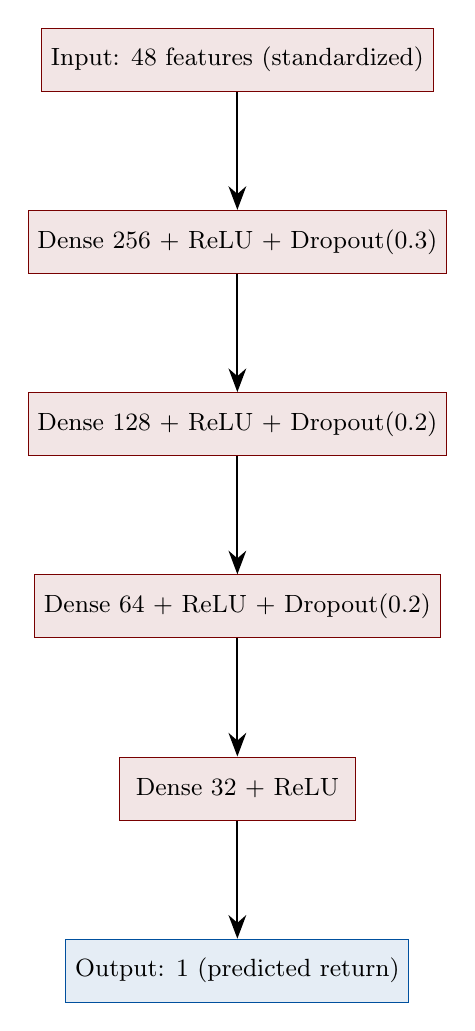
\begin{tikzpicture}[
    node distance=1.5cm,
    layer/.style={rectangle, draw=metu, fill=metu!10, minimum width=3cm, minimum height=0.8cm, font=\small},
    arrow/.style={-{Stealth[length=3mm]}, thick}
]
\node[layer] (input) {Input: 48 features (standardized)};
\node[layer, below=of input] (h1) {Dense 256 + ReLU + Dropout(0.3)};
\node[layer, below=of h1] (h2) {Dense 128 + ReLU + Dropout(0.2)};
\node[layer, below=of h2] (h3) {Dense 64 + ReLU + Dropout(0.2)};
\node[layer, below=of h3] (h4) {Dense 32 + ReLU};
\node[layer, below=of h4, fill=accentblue!10, draw=accentblue] (output) {Output: 1 (predicted return)};

\draw[arrow] (input) -- (h1);
\draw[arrow] (h1) -- (h2);
\draw[arrow] (h2) -- (h3);
\draw[arrow] (h3) -- (h4);
\draw[arrow] (h4) -- (output);
\end{tikzpicture}
\caption{Feedforward neural network architecture.}
\end{figure}

\textbf{Training details:}
\begin{itemize}[nosep]
    \item Loss: Mean Squared Error (MSE) for regression; Binary Cross-Entropy for classification
    \item Optimizer: Adam with initial learning rate $10^{-3}$
    \item Learning rate schedule: ReduceLROnPlateau (patience=5, factor=0.5)
    \item Early stopping: Patience of 10 epochs on validation loss
    \item Batch size: 256
    \item Input standardization: Zero mean, unit variance (computed on training set only)
\end{itemize}

\subsection{Model 2: XGBoost}

Gradient-boosted decision trees, trained on the same feature set. XGBoost serves as both a competitive baseline and a source of \emph{exact} SHAP values via TreeExplainer.

\textbf{Hyperparameters (tuned via Bayesian optimization):}
\begin{itemize}[nosep]
    \item \texttt{max\_depth}: 4--8
    \item \texttt{learning\_rate}: 0.01--0.1
    \item \texttt{n\_estimators}: 500--2000 (with early stopping)
    \item \texttt{subsample}: 0.7--0.9
    \item \texttt{colsample\_bytree}: 0.7--0.9
    \item \texttt{reg\_alpha}, \texttt{reg\_lambda}: L1/L2 regularization
\end{itemize}

\subsection{Model 3: Temporal Fusion Transformer (TFT)}

The TFT (Lim et al., 2021) is designed for multi-horizon time series forecasting with built-in interpretability. Its key components:

\begin{figure}[H]
\centering
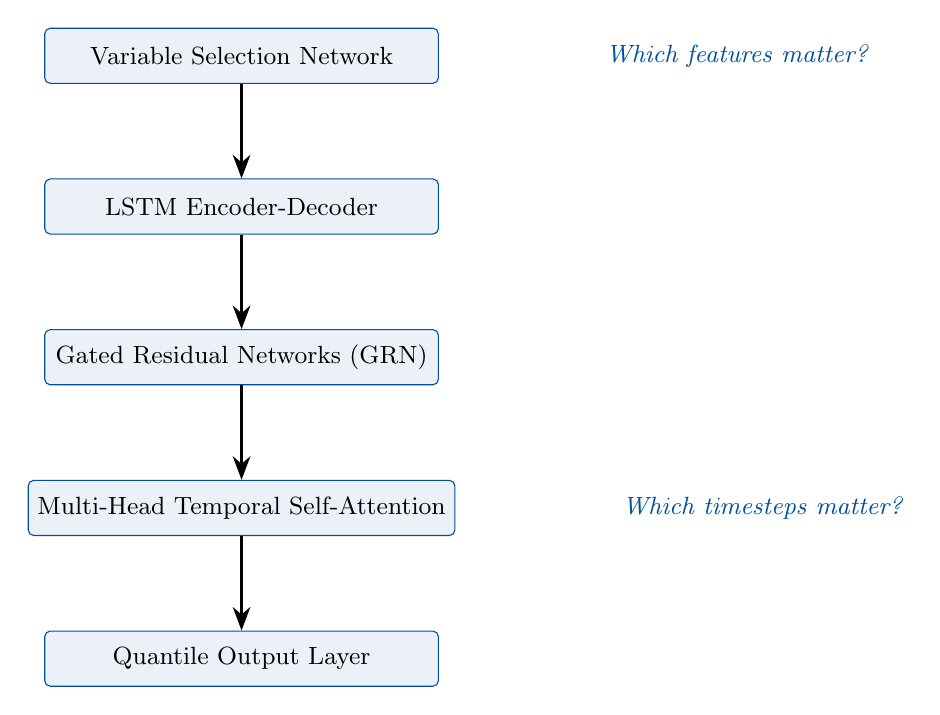
\begin{tikzpicture}[
    node distance=1.2cm,
    block/.style={rectangle, draw=accentblue, fill=accentblue!8, minimum width=5cm, minimum height=0.7cm, font=\small, rounded corners=2pt},
    arrow/.style={-{Stealth[length=3mm]}, thick}
]
\node[block] (vsn) {Variable Selection Network};
\node[block, below=of vsn] (lstm) {LSTM Encoder-Decoder};
\node[block, below=of lstm] (grn) {Gated Residual Networks (GRN)};
\node[block, below=of grn] (attn) {Multi-Head Temporal Self-Attention};
\node[block, below=of attn] (quant) {Quantile Output Layer};

\draw[arrow] (vsn) -- (lstm);
\draw[arrow] (lstm) -- (grn);
\draw[arrow] (grn) -- (attn);
\draw[arrow] (attn) -- (quant);

\node[right=2cm of vsn, font=\small\itshape, text=accentblue] {Which features matter?};
\node[right=2cm of attn, font=\small\itshape, text=accentblue] {Which timesteps matter?};
\end{tikzpicture}
\caption{Temporal Fusion Transformer architecture (simplified).}
\end{figure}

\textbf{Why TFT is ideal for this project:}
\begin{itemize}[nosep]
    \item \textbf{Variable Selection Networks} learn which features are important, providing a learned (not post-hoc) feature importance ranking that can be directly compared to SHAP.
    \item \textbf{Temporal self-attention} shows which past days the model attends to, revealing the effective ``memory'' for each feature.
    \item \textbf{Separate static vs.\ time-varying feature handling}: Ticker identity and sector are static; IV changes and volume are time-varying. TFT handles this distinction natively.
    \item \textbf{Quantile regression output}: Directly produces prediction intervals (10th, 50th, 90th percentiles), providing built-in uncertainty quantification without requiring conformal prediction as a separate step.
\end{itemize}

\textbf{Input configuration for TFT:}
\begin{itemize}[nosep]
    \item Lookback window: 20 trading days (one month of history)
    \item Static covariates: Ticker (categorical), sector (categorical)
    \item Time-varying known inputs: Day of week, days to earnings, days to OpEx, quarter-end flag
    \item Time-varying observed inputs: All options-derived features + stock features
\end{itemize}

\subsection{Model 4: TabNet}

TabNet (Arik \& Pfister, 2021) uses sequential attention to decide which features to use at each decision step. Key properties:

\begin{itemize}[nosep]
    \item \textbf{Instance-wise feature selection}: For each prediction, TabNet produces an attention mask showing which features it ``looked at.'' This enables per-prediction explainability.
    \item \textbf{Sparsity}: The attention mechanism is regularized to be sparse, meaning the model uses only a subset of features for each prediction. This mirrors how an experienced trader might focus on different signals depending on market conditions.
    \item \textbf{No preprocessing required}: TabNet handles raw features without standardization.
\end{itemize}

\subsection{Benchmark Models}

\begin{itemize}[nosep]
    \item \textbf{Na\"ive baseline}: Predict $r_{t+1} = 0$ (random walk hypothesis). Equivalent to predicting tomorrow's price equals today's price.
    \item \textbf{Historical mean}: Predict $r_{t+1} = \bar{r}$ (average historical return for that stock).
    \item \textbf{Linear regression (OLS)}: On the full feature set. Tests whether the relationship is linear.
    \item \textbf{Linear regression (BS inputs only)}: On only the 5 Black--Scholes-related features. Establishes the baseline explanatory power of classical inputs.
\end{itemize}


% ════════════════════════════════════════
% 6. EXPERIMENTAL DESIGN
% ════════════════════════════════════════
\section{Experimental Design}

\subsection{The Three-Model Comparison: Isolating Options Information Value}

The core experiment compares three feature sets to isolate the marginal predictive value of options data:

\begin{table}[H]
\centering
\begin{tabularx}{\textwidth}{@{}lXl@{}}
\toprule
\textbf{Experiment} & \textbf{Features Used} & \textbf{Question Answered} \\
\midrule
Model A & Stock features only (\#27--42) & How well can we predict with equity data alone? \\
Model B & Options features only (\#1--26) & Can the options market alone predict stock returns? \\
Model C & All features (\#1--49) & Does combining both improve prediction? \\
\bottomrule
\end{tabularx}
\caption{Three-model comparison design.}
\end{table}

\begin{keyinsight}
The difference in performance between Models A and C quantifies the \textbf{marginal predictive value of options market information}. The comparison between Models A and B reveals \textbf{which information source is more powerful on its own}. Both comparisons produce interesting findings regardless of the outcome.
\end{keyinsight}

\subsection{Temporal Train / Validation / Test Split}

\begin{warningbox}
Data is split \emph{temporally}, never randomly. Random splitting in financial time series creates information leakage---the model implicitly sees future data during training---which inflates performance metrics and produces results that do not generalize. This is a common error in financial ML research.
\end{warningbox}

\textbf{Primary split} (for main results):
\begin{itemize}[nosep]
    \item Training: Earliest 60\% of the data
    \item Validation: Next 20\% (for hyperparameter tuning and early stopping)
    \item Test: Most recent 20\% (never touched until final evaluation)
\end{itemize}

\textbf{Rolling-window evaluation} (for robustness):
\begin{itemize}[nosep]
    \item Train on months 1--6, validate on month 7, test on month 8
    \item Roll forward: train on months 2--7, validate on month 8, test on month 9
    \item Continue until end of data
    \item Report mean and standard deviation of metrics across all windows
\end{itemize}

The rolling-window approach tests whether the model's performance is stable over time or concentrated in specific periods. If performance varies wildly across windows, the predictability may be regime-dependent---which is itself an interesting finding for the SHAP analysis.

\subsection{Comparison with Known Single-Signal Predictors}

To establish that our multi-feature model captures information beyond established predictors, we also evaluate:
\begin{itemize}[nosep]
    \item Put-call ratio alone (Pan \& Poteshman, 2006)
    \item IV change alone (An \& Ang, 2012)
    \item Put-call parity deviation (Cremers \& Weinbaum, 2010)
\end{itemize}
each implemented as simple linear predictors. If the full model outperforms these, it demonstrates that the \emph{combination and nonlinear interaction} of options signals carries information that individual signals miss.


% ════════════════════════════════════════
% 7. EXPLAINABILITY FRAMEWORK
% ════════════════════════════════════════
\section{Explainability Framework}

This is the core intellectual contribution of the project. We employ three complementary explainability methods, cross-validated against each other.

\subsection{SHAP (SHapley Additive exPlanations)}

SHAP decomposes each prediction into additive feature contributions based on Shapley values from cooperative game theory:
\begin{equation}
\hat{y}_i = \phi_0 + \sum_{j=1}^{d} \phi_j^{(i)}
\end{equation}
where $\phi_0$ is the base value (mean prediction) and $\phi_j^{(i)}$ is the contribution of feature $j$ to prediction $i$.

\textbf{Properties:}
\begin{itemize}[nosep]
    \item \textbf{Local accuracy}: SHAP values sum exactly to the prediction.
    \item \textbf{Consistency}: If a model changes so that a feature's contribution increases, its SHAP value does not decrease.
    \item \textbf{Missingness}: Features with no impact receive a SHAP value of zero.
\end{itemize}

\textbf{Implementation:}
\begin{itemize}[nosep]
    \item \texttt{shap.TreeExplainer} for XGBoost (exact Shapley values, fast)
    \item \texttt{shap.DeepExplainer} or \texttt{shap.GradientExplainer} for the feedforward NN (approximate)
    \item \texttt{shap.KernelExplainer} as a model-agnostic backup
\end{itemize}

\textbf{Analyses performed:}
\begin{enumerate}[nosep]
    \item \textbf{Global feature importance}: Mean absolute SHAP value across all test predictions, ranked.
    \item \textbf{SHAP summary (beeswarm) plots}: Show the distribution of SHAP values for each feature, revealing not just importance but also direction (positive/negative impact).
    \item \textbf{SHAP dependence plots}: Show how the SHAP value of a feature varies with its actual value, revealing nonlinear relationships and threshold effects.
    \item \textbf{SHAP interaction values}: Identify the most important feature pairs, revealing synergistic effects (e.g., does IV change matter more when the earnings flag is active?).
    \item \textbf{Local explanations}: For specific high-residual predictions, show exactly which features drove the model's output.
\end{enumerate}

\subsection{TFT Variable Selection and Attention Weights}

The TFT provides two built-in interpretability mechanisms:

\textbf{Variable importance weights}: The Variable Selection Network outputs a softmax-normalized weight for each input feature, learned end-to-end during training. These weights represent the model's learned assessment of each feature's relevance.

\textbf{Temporal attention patterns}: The multi-head self-attention layer produces attention weights over the lookback window. These reveal which historical days the model considers most relevant for each prediction. For example, we may find that the model attends heavily to the day before earnings (capturing the final pre-announcement positioning) or to days with unusual volume spikes.

\subsection{TabNet Attention Masks}

TabNet produces instance-wise feature attention masks at each decision step. Aggregating these masks across the test set reveals:
\begin{itemize}[nosep]
    \item Which features TabNet uses most frequently
    \item Whether feature usage patterns cluster into interpretable ``strategies''
    \item How feature attention shifts across different market conditions
\end{itemize}

\subsection{Cross-Validation of Explainability Methods}

\begin{keyinsight}
By comparing SHAP rankings (post-hoc), TFT variable selection weights (learned, temporal), and TabNet attention masks (learned, instance-wise), we can assess the \textbf{robustness of our feature importance findings}. Features that rank highly across all three methods are genuinely important; features that rank highly in one method but not others may reflect method-specific artifacts.
\end{keyinsight}


% ════════════════════════════════════════
% 8. REGIME-CONDITIONAL ANALYSIS
% ════════════════════════════════════════
\section{Regime-Conditional Analysis}

The global analysis tells us which features matter \emph{on average}. The regime-conditional analysis asks: \textbf{does this change when market conditions change?} This is where the most publishable findings will emerge.

\subsection{Regime Definitions}

\begin{table}[H]
\centering
\begin{tabularx}{\textwidth}{@{}lXX@{}}
\toprule
\textbf{Regime Split} & \textbf{Condition A} & \textbf{Condition B} \\
\midrule
Volatility regime & High VIX ($>$25) & Low VIX ($<$15) \\
Earnings proximity & Pre-earnings (within 7 days) & Normal period \\
Options liquidity & High liquidity (top quartile volume) & Low liquidity (bottom quartile) \\
Market trend & Bullish (20-day return $>$0) & Bearish (20-day return $<$0) \\
Dealer positioning & Positive GEX (vol-suppressing) & Negative GEX (vol-amplifying) \\
\bottomrule
\end{tabularx}
\caption{Regime splits for conditional analysis.}
\end{table}

\subsection{Expected Findings and Hypotheses}

For each regime split, we compute SHAP feature importance separately for each condition and compare. Specific hypotheses:

\textbf{Volatility regime:} In high-VIX environments, we expect liquidity features (bid-ask spread, volume, open interest) to become more important, because liquidity dries up and the premium for it grows. IV-related features may become less informative because IV is already elevated and less discriminating.

\textbf{Earnings proximity:} In the pre-earnings window, we expect days-to-earnings, IV change, and unusual activity features to spike in importance. The options market should contain more predictive information about the stock around earnings, because informed traders position in options before announcements. If this hypothesis is confirmed, it provides direct evidence of information leakage through the options market.

\textbf{Options liquidity:} For stocks with very liquid options markets (SPY, AAPL), price discovery may happen simultaneously in both markets, diluting the predictive power of options signals. For less liquid options, information may take longer to propagate from options to stocks, creating a stronger predictive relationship.

\textbf{Dealer positioning:} When GEX is negative (dealers short gamma), stock movements are amplified by hedging flows. Options-derived directional signals (put-call ratio, net delta) may be more predictive in this regime because the mechanical feedback loop magnifies the initial signal. When GEX is positive, the dampening effect may reduce directional predictability.


% ════════════════════════════════════════
% 9. EVALUATION METRICS
% ════════════════════════════════════════
\section{Evaluation Metrics and Statistical Testing}

\subsection{Regression Metrics}

\begin{table}[H]
\centering
\begin{tabular}{@{}lll@{}}
\toprule
\textbf{Metric} & \textbf{Formula} & \textbf{Purpose} \\
\midrule
RMSE & $\sqrt{\frac{1}{n}\sum_{i=1}^{n}(\hat{r}_i - r_i)^2}$ & Penalizes large errors \\[6pt]
MAE & $\frac{1}{n}\sum_{i=1}^{n}|\hat{r}_i - r_i|$ & Robust to outliers \\[6pt]
$R^2$ & $1 - \frac{\sum(\hat{r}_i - r_i)^2}{\sum(r_i - \bar{r})^2}$ & Variance explained \\[6pt]
OOS $R^2$ & $1 - \frac{\sum(\hat{r}_i - r_i)^2}{\sum r_i^2}$ & Campbell \& Thompson (2008) \\
\bottomrule
\end{tabular}
\caption{Regression evaluation metrics. OOS $R^2$ uses zero as the benchmark (random walk).}
\end{table}

The out-of-sample $R^2$ of Campbell and Thompson (2008) is the standard metric in financial return prediction. It compares the model's forecast error to the simple forecast of zero (random walk). An OOS $R^2$ of 0.01--0.05 at the daily frequency is considered economically significant.

\subsection{Classification Metrics}

For the direction prediction variant: Accuracy, Precision, Recall, F1-score, AUC-ROC, and the hit rate (fraction of correctly predicted positive/negative return days).

\subsection{Statistical Significance Tests}

\textbf{Diebold-Mariano test}: Tests whether the difference in forecast errors between two models is statistically significant. Applied to every pairwise model comparison.

\textbf{Clark-West test}: Specifically designed for nested models (e.g., Model A is nested within Model C). Tests whether the larger model's improvement is significant after correcting for the noise introduced by estimating additional parameters.

\textbf{Bootstrap confidence intervals}: For SHAP feature importance rankings. We bootstrap-resample the test set 1000 times, compute SHAP rankings each time, and report 95\% confidence intervals for each feature's rank.


% ════════════════════════════════════════
% 10. UNCERTAINTY QUANTIFICATION
% ════════════════════════════════════════
\section{Uncertainty Quantification via Conformal Prediction}

\subsection{Motivation}

A point prediction of ``the stock will return +0.3\% tomorrow'' is practically useless without a measure of confidence. Conformal prediction (Vovk et al., 2005) provides distribution-free prediction intervals with guaranteed finite-sample coverage.

\subsection{Method}

Split conformal prediction is applied as follows:

\begin{enumerate}[nosep]
    \item Split the validation set into a proper training set and a calibration set.
    \item Fit the model on the proper training set.
    \item Compute residuals $|r_i - \hat{r}_i|$ on the calibration set.
    \item Sort residuals and find the $\lceil (1-\alpha)(1 + 1/n) \rceil$-th smallest value, call it $q$.
    \item For any new prediction $\hat{r}_{\text{new}}$, the prediction interval is $[\hat{r}_{\text{new}} - q, \hat{r}_{\text{new}} + q]$.
\end{enumerate}

This guarantees at least $(1-\alpha)$ coverage on the test set, regardless of the model or data distribution.

\subsection{Use in This Project}

We analyze how prediction interval width varies across regimes:
\begin{itemize}[nosep]
    \item Wider intervals before earnings (the model ``knows'' it is uncertain)
    \item Narrower intervals in low-VIX environments
    \item Wider intervals for stocks with illiquid options
\end{itemize}

This also provides a natural \textbf{trading filter}: only act on predictions where the interval is narrow (high confidence). We report separate performance metrics for the ``confident'' subset.


% ════════════════════════════════════════
% 11. DATA PIPELINE
% ════════════════════════════════════════
\section{Data Pipeline}

\subsection{Data Sources}

\begin{table}[H]
\centering
\begin{tabularx}{\textwidth}{@{}lXl@{}}
\toprule
\textbf{Data Type} & \textbf{Source Options} & \textbf{Fields Needed} \\
\midrule
Options chains (EOD) & CBOE DataShop, OptionMetrics (WRDS), Polygon.io, ORATS & Strike, expiry, bid, ask, last, volume, OI, IV, Greeks \\
Stock prices (EOD) & Yahoo Finance, Polygon.io, Alpha Vantage & OHLCV, adjusted close \\
VIX \& VIX3M & CBOE, Yahoo Finance & Daily close \\
Earnings dates & Nasdaq Earnings Calendar, SEC EDGAR, Alpha Vantage & Announcement dates \\
Dividend dates & Yahoo Finance, Alpha Vantage & Ex-dividend dates \\
Risk-free rate & FRED (3-month T-bill) & Daily yield \\
Sector ETFs & Yahoo Finance & Daily returns \\
News headlines & Financial news APIs (for LLM sentiment) & Headline text, timestamp \\
\bottomrule
\end{tabularx}
\caption{Data sources and required fields.}
\end{table}

\subsection{Ticker Universe}

\begin{table}[H]
\centering
\begin{tabular}{@{}lll@{}}
\toprule
\textbf{Ticker} & \textbf{Name} & \textbf{Sector / Why Included} \\
\midrule
SPY & S\&P 500 ETF & Most liquid options globally; broad market \\
QQQ & Nasdaq-100 ETF & Tech-heavy; second most liquid \\
AAPL & Apple & Mega-cap tech; extremely liquid options \\
TSLA & Tesla & High-volatility; retail-dominated options activity \\
NVDA & NVIDIA & AI/semiconductor exposure; high recent vol \\
AMZN & Amazon & Consumer/tech; diverse options chain \\
META & Meta Platforms & Social media; event-driven (earnings) \\
MSFT & Microsoft & Stable mega-cap; institutional-dominated \\
GOOGL & Alphabet & Large-cap tech \\
JPM & JPMorgan Chase & Financials; different sector dynamics \\
\bottomrule
\end{tabular}
\caption{Ticker universe with selection rationale.}
\end{table}

\subsection{Data Filtering Rules}

Applied at the contract level before aggregation:
\begin{enumerate}[nosep]
    \item Remove contracts with open interest $\leq 10$
    \item Remove contracts with bid $= 0$ (no active market)
    \item Remove contracts with moneyness outside $[0.80, 1.20]$
    \item Remove contracts with fewer than 7 DTE (dominated by expiration noise)
    \item Remove contracts where last trade price is outside bid-ask range by $>$10\%
\end{enumerate}

\subsection{Pipeline Architecture}

\begin{figure}[H]
\centering
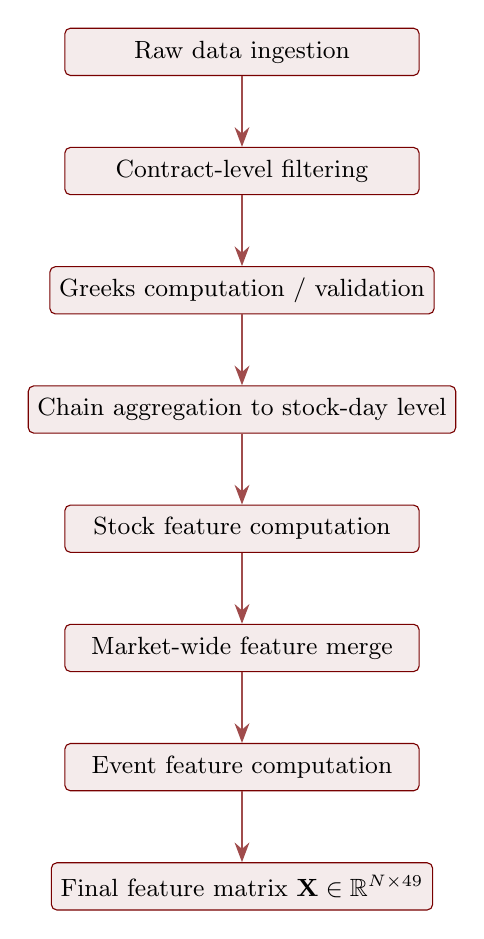
\begin{tikzpicture}[
    node distance=0.9cm,
    pipestep/.style={rectangle, draw=metu, fill=metu!8, minimum width=4.5cm, minimum height=0.6cm, font=\small, rounded corners=2pt},
    arrow/.style={-{Stealth[length=2.5mm]}, thick, metu!70}
]
\node[pipestep] (raw) {Raw data ingestion};
\node[pipestep, below=of raw] (filter) {Contract-level filtering};
\node[pipestep, below=of filter] (greeks) {Greeks computation / validation};
\node[pipestep, below=of greeks] (agg) {Chain aggregation to stock-day level};
\node[pipestep, below=of agg] (stock) {Stock feature computation};
\node[pipestep, below=of stock] (market) {Market-wide feature merge};
\node[pipestep, below=of market] (event) {Event feature computation};
\node[pipestep, below=of event] (final) {Final feature matrix $\mathbf{X} \in \mathbb{R}^{N \times 49}$};

\draw[arrow] (raw) -- (filter);
\draw[arrow] (filter) -- (greeks);
\draw[arrow] (greeks) -- (agg);
\draw[arrow] (agg) -- (stock);
\draw[arrow] (stock) -- (market);
\draw[arrow] (market) -- (event);
\draw[arrow] (event) -- (final);
\end{tikzpicture}
\caption{Data pipeline from raw options chains to final feature matrix.}
\end{figure}


% ════════════════════════════════════════
% 12. ECONOMIC SIGNIFICANCE
% ════════════════════════════════════════
\section{Economic Significance Analysis}

\subsection{Simple Trading Strategy}

To assess whether statistical predictability translates to economic value, we construct a simple long-short strategy:

\begin{enumerate}[nosep]
    \item Each day, rank all 10 stocks by predicted next-day return.
    \item Go long the top 3 (highest predicted return) and short the bottom 3 (lowest predicted return), equal-weighted.
    \item Compute daily portfolio return. Report annualized return, Sharpe ratio, and maximum drawdown.
\end{enumerate}

\subsection{Transaction Cost Analysis}

We report results both gross and net of transaction costs:
\begin{itemize}[nosep]
    \item Assume 5 basis points (0.05\%) per trade as a conservative estimate for large-cap US equities.
    \item Report the \emph{break-even} transaction cost: the cost level at which the strategy's net Sharpe ratio drops to zero.
\end{itemize}

\subsection{Confidence-Filtered Trading}

Using conformal prediction intervals, we also report a filtered strategy that only trades when the prediction interval is in the narrowest quartile (highest confidence). This tests whether the model's uncertainty awareness translates into better risk-adjusted returns.


% ════════════════════════════════════════
% 13. POTENTIAL FINDINGS
% ════════════════════════════════════════
\section{Potential Findings and Contributions}

\subsection{Expected Contributions}

\begin{enumerate}
    \item \textbf{Comprehensive feature importance ranking} for options-based equity return prediction, identifying which observable options variables are most predictive of stock returns---and crucially, which are \emph{not} informative despite common belief.
    
    \item \textbf{Marginal value quantification} of options market information for stock return prediction, established through the Model A/B/C comparison and formal statistical tests.
    
    \item \textbf{Regime-conditional analysis} showing how the information channel between options and stocks shifts across volatility regimes, earnings cycles, liquidity conditions, and dealer positioning. This is the core contribution.
    
    \item \textbf{Cross-method explainability validation} comparing SHAP (post-hoc), TFT variable selection (learned temporal), and TabNet attention (learned instance-wise) to assess robustness.
    
    \item \textbf{Dealer gamma exposure as a predictor}: If GEX shows up as important in SHAP, this provides evidence that the \emph{mechanical} structure of the options market (not just informational content) affects stock prices.
    
    \item \textbf{Practical benchmark} comparing classical statistics, gradient boosting, feedforward networks, and modern temporal architectures for financial return prediction.
\end{enumerate}

\subsection{Risk: Null Results}

\begin{warningbox}
There is a non-trivial probability that options features do not significantly improve stock return prediction after controlling for stock-level information. This would be a valid and publishable null result---it would mean that whatever information exists in the options market is already incorporated into stock prices sufficiently fast that end-of-day options data carries no residual predictive power. However, even in this scenario, the regime-conditional analysis and the cross-method explainability comparison remain valuable contributions.
\end{warningbox}


% ════════════════════════════════════════
% 14. TECHNICAL STACK
% ════════════════════════════════════════
\section{Technical Implementation}

\subsection{Software Stack}

\begin{table}[H]
\centering
\begin{tabular}{@{}ll@{}}
\toprule
\textbf{Component} & \textbf{Library / Tool} \\
\midrule
Data processing & Pandas, NumPy, Polars \\
Feature engineering & Custom Python (TA-Lib for technicals) \\
Neural network & PyTorch \\
XGBoost & XGBoost Python API \\
TFT & PyTorch Forecasting / Darts \\
TabNet & pytorch-tabnet \\
SHAP analysis & shap (Python library) \\
Conformal prediction & MAPIE or custom implementation \\
LLM sentiment & HuggingFace Transformers (FinBERT) \\
Visualization & Matplotlib, Seaborn, Plotly \\
Experiment tracking & Weights \& Biases (wandb) \\
Version control & Git \\
\bottomrule
\end{tabular}
\caption{Technical stack.}
\end{table}


% ════════════════════════════════════════
% 15. TIMELINE
% ════════════════════════════════════════
\section{Project Timeline}

\begin{table}[H]
\centering
\begin{tabularx}{\textwidth}{@{}lX@{}}
\toprule
\textbf{Period} & \textbf{Tasks} \\
\midrule
Weeks 1--3 & Data acquisition, pipeline construction, contract filtering, chain aggregation. Feature engineering for all 49 features. Exploratory data analysis. \\
\addlinespace
Weeks 4--5 & Implement and train feedforward NN and XGBoost. Run Model A/B/C comparison. Compute baseline metrics. \\
\addlinespace
Weeks 6--7 & Implement TFT and TabNet. Hyperparameter tuning via Bayesian optimization. Rolling-window evaluation. \\
\addlinespace
Weeks 8--9 & SHAP analysis: global importance, beeswarm plots, dependence plots, interaction values. TFT variable selection extraction. TabNet attention mask analysis. \\
\addlinespace
Weeks 10--11 & Regime-conditional SHAP analysis across all five regime splits. Cross-method comparison. Conformal prediction implementation. \\
\addlinespace
Weeks 12--13 & Economic significance analysis (trading strategy, transaction costs). LLM sentiment feature (if time permits). Statistical testing (Diebold-Mariano, Clark-West, bootstrap). \\
\addlinespace
Week 14 & Final report writing, figure generation, results synthesis. \\
\bottomrule
\end{tabularx}
\caption{14-week project timeline.}
\end{table}


% ════════════════════════════════════════
% 16. FUTURE EXTENSIONS
% ════════════════════════════════════════
\section{Future Extensions}

\subsection{Graph Neural Networks for Cross-Asset Information Flow}

The 10 tickers in our universe do not exist in isolation. NVDA options activity might predict AAPL stock movement because of shared supply chain exposure. A GNN can model these cross-asset dependencies:

\begin{itemize}[nosep]
    \item \textbf{Nodes}: Stocks. Node features: options-derived variables.
    \item \textbf{Edges}: Initialized from sector membership or return correlations.
    \item \textbf{Learning}: The GNN learns whether unusual options activity in one stock propagates predictive information to related stocks.
\end{itemize}

This is genuinely novel and would strengthen the paper for a top-tier venue.

\subsection{Intraday Analysis}

Using intraday options data (5-minute intervals from OPRA), we could analyze the speed of information flow from options to stocks. How quickly are options signals incorporated into stock prices? Does this speed vary by regime?

\subsection{Expanded Universe}

Extending from 10 to 50--100 stocks would enable cross-sectional analysis: are options signals more predictive for certain types of stocks (small-cap vs.\ large-cap, high-beta vs.\ low-beta)?

\subsection{Causal Identification}

Moving from prediction to causal inference---showing that options activity \emph{causes} stock price movement rather than merely correlating with it---would require instrumental variables or natural experiments. This is the most challenging extension but would qualify the work for a top-tier finance journal.


% ════════════════════════════════════════
% 17. REFERENCES
% ════════════════════════════════════════
\section{Key References}

\begin{enumerate}[nosep, label={[\arabic*]}]
    \item An, B.~J., \& Ang, A. (2012). ``Implied volatility and future stock returns.'' Working paper.
    \item Arik, S.~\"O., \& Pfister, T. (2021). ``TabNet: Attentive interpretable tabular learning.'' \textit{AAAI}.
    \item Bakshi, G., Kapadia, N., \& Madan, D. (2003). ``Stock return characteristics, skew laws, and differential pricing of individual equity options.'' \textit{Review of Financial Studies}, 16(1), 101--143.
    \item Black, F., \& Scholes, M. (1973). ``The pricing of options and corporate liabilities.'' \textit{Journal of Political Economy}, 81(3), 637--654.
    \item Campbell, J.~Y., \& Thompson, S.~B. (2008). ``Predicting excess stock returns out of sample.'' \textit{Review of Financial Studies}, 21(4), 1509--1531.
    \item Cremers, M., \& Weinbaum, D. (2010). ``Deviations from put-call parity and stock return predictability.'' \textit{Journal of Financial and Quantitative Analysis}, 45(2), 335--367.
    \item Easley, D., O'Hara, M., \& Srinivas, P.~S. (1998). ``Option volume and stock prices.'' \textit{Journal of Finance}, 53(2), 431--465.
    \item Lim, B., Ar\i k, S.~\"O., Loeff, N., \& Pfister, T. (2021). ``Temporal fusion transformers for interpretable multi-horizon time series forecasting.'' \textit{International Journal of Forecasting}, 37(4), 1748--1764.
    \item Lundberg, S.~M., \& Lee, S.~I. (2017). ``A unified approach to interpreting model predictions.'' \textit{NeurIPS}.
    \item Pan, J., \& Poteshman, A.~M. (2006). ``The information in option volume for future stock prices.'' \textit{Review of Financial Studies}, 19(3), 871--908.
    \item Vovk, V., Gammerman, A., \& Shafer, G. (2005). \textit{Algorithmic Learning in a Random World}. Springer.
\end{enumerate}

\vspace{1cm}
\begin{center}
\textcolor{metu}{\rule{0.5\textwidth}{1pt}}\\[0.5cm]
{\large\textcolor{metu}{End of Document}}
\end{center}

\end{document}